\documentclass{article}
\usepackage[T1]{fontenc}
\usepackage{graphicx}
\usepackage{amsthm}
\usepackage{amsmath}
\usepackage{mathtools}
\usepackage{xcolor}
\usepackage{footnote}
\usepackage{hyperref}
\hypersetup{colorlinks=True,
            linkcolor=brown}
\usepackage{subcaption}
\usepackage{caption}
\usepackage{amssymb}
\usepackage{calrsfs}

\begin{document}

\title{Notes on ARIMA in MLCore}
\author{Solidware}
\date{10 November 2019}
\maketitle


\section{ARMA}

Given a centred time series $y=y_1, \ldots, y_n$ of finite rank, ARIMA(p, d=0, q) equation is:

\begin{equation}
  \label{eq1}
y_{t+1}=\mu(=0)+\epsilon_{t+1}+\Sigma_{i=1}^{q}\theta_{i}\epsilon_{t-i+1}+\Sigma_{i=1}^{p}\alpha_{i}y_{t-i+1} 
\end{equation}

where $\epsilon^{(h)}$ is the series of residuals referring to the $h$-th target\footnote{here, "target" is to be taken in the scope of a prediction horizon: we do consider a unique "target time series", $y$ but one may be interested in predicting multiple ($h$) steps ahead: $y_{t+1}, y_{t+2}, \dots, y_{t+h}$, or more generally $y_{t+g+1},\dots, y_{t+g+h+1}, \forall g\geq 0, h>0$.}, $y_{t+h}$ (only 1 step ahead is used here, so the superscript was dropped for clarity). 

The first part (in $\epsilon$) is the MA(q) model and the last sum (in $y$) corresponds to the AR(p) model. As a side note, one could verify that the residuals are not correlated and iid variables sampled from a normal distribution with 0 mean.

It is also worth mentioning that we restricted ourselves to a (prediction) gap, g=0 here and used a non-differentiated series\footnote{when using ARIMA(p, d>0, q), $y$ and $x$ are replaced with their differentiated versions in (\ref{eq2}). One could also encounter the lag operator $\mathcal{L}$ in the literature, which, when applied to $y$ simply gives $\mathcal{L}^iy_t=y_{t-i}$ (it just avoids carrying all the $t-i+1$ indices along); besides, note that $(1-\mathcal{L}^1)y_t=y_t-y_{t-1}$. For $d>0$, $g=0$, (\ref{eq1}) can therefore be rewritten as: $\big(1-\sum_{i=1}^p \alpha_i \mathcal{L}^i \big) (1-\mathcal{L}^1)^dy_{t+1} = \big(1-\sum_{i=1}^q \theta_i \mathcal{L}^i \big)\epsilon_{t+1}$; see Section~\ref{diff} for more details.} (d=0) without any additional (exogenous) data; in such case, given k exogenous series $x^{(k)}$ ($y$ still being our endogenous, unique target series) and a non-null gap, eq.~(\ref{eq1}) just becomes:
\begin{equation}
\begin{split}
\label{eq2}
y_{t+g+1} = \epsilon_{t+g+1} + f(\epsilon_{t}, \dots, \epsilon_{t-q+1}, y_{t},\dots, y_{t-p+1}, x^{(1)}_{t}, \dots, x^{(1)}_{t-p+1}, \dots, \\
x^{(k)}_{t}, \dots, x^{(k)}_{t-p+1}, \theta, \alpha)
\end{split}
\end{equation}
where $f$ is a polynomial function of degree 1 with more variables and coefficient sets $\theta$ and $\alpha$ (referring to MA and AR respectively).


\subsection{Difference with the classical ARIMA}
When $q>0$, we do not compute the series of residuals \textbf{exactly}, like in the classical MA model (i.e. via backward recursion). The reason is that in order to compute a residual, one needs a target (so $q+h$ observations)...but this is not always possible (e.g. at the end of the series). So instead, we rather estimate a residual series $\hat{\epsilon}$, at once, from the set of all $q$ consecutive observations available via a linear predictor (see {\fontfamily{pcr}\selectfont ResidualPredictor}), and use it in eq.~(\ref{eq1}). The ARMA equation thus becomes: 

$$ y_{t+1} - \hat{\epsilon}_{t+1} = \underbrace{\Sigma_{i=1}^{q}\theta_{i} \hat{\epsilon}_{t-i+1} + \Sigma_{i=1}^{p}\alpha_{i} y_{t-i+1}}_{\widetilde{y}_{t+1}}$$


% For example, taking $p=3$ and $q=4$, we get:
% \begin{align}
% y_5 &= \hat{\epsilon}_{5} + \Sigma_{i=1}^{4}\theta_i \hat{\epsilon}_{5-i} + \Sigma_{i=1}^{3}\alpha_i y_{5-i}\nonumber \\
% &= \hat{\epsilon}_{5} + \alpha_4 y_4 + \alpha_3 y_3 + \alpha_2 y_2\nonumber
% \end{align}


Therefore, we seek $\mathbf{\alpha}$ and $\mathbf{\theta}$ that minimise:
$$\textmd{argmin}_{\mathbf{\alpha}, \Theta} \Sigma_{t>\text{max}(p,2q)} \Big[ (y_{t+1}-\hat{\epsilon}_{t+1}) - \widetilde{y}_{t+1}\Big]^2$$


\subsection{ARIMA(p, 0, q)}

In general (though here, exogenous features were excluded for clarity), this means that the "feature-target" matrix, $X$ (with h=2 targets) fed to the final linear model (within the {\fontfamily{pcr}\selectfont fit} method of the class {\fontfamily{pcr}\selectfont ARIMA}) has the form:

$$\tiny\left[\begin{array}{ccc|cccc|cccc|cc}
  \centering
  . & . & .  & . & . & . & . & . & . & . & . & . & y_1-\textcolor{red}{\hat{\epsilon}_1^{(2)}} \\
. & . & .  & . & . & . & . & . & . & . & . &  y_1-\textcolor{red}{\hat{\epsilon}_1^{(1)}} & y_2-\textcolor{red}{\hat{\epsilon}_2^{(2)}} \\
. & . & y_1  & . & . & . & \textcolor{red}{\hat{\epsilon}_1^{(1)}} & . & . & . & \textcolor{red}{\hat{\epsilon}_1^{(2)}} & y_2-\textcolor{red}{\hat{\epsilon}_2^{(1)}} & y_3-\textcolor{red}{\hat{\epsilon}_3^{(2)}}\\
. & y_1 & y_2  & . & . & \textcolor{red}{\hat{\epsilon}_1^{(1)}} & \textcolor{red}{\hat{\epsilon}_2^{(1)}} & . & . & \textcolor{red}{\hat{\epsilon}_1^{(2)}} & \textcolor{red}{\hat{\epsilon}_2^{(2)}} & y_3-\textcolor{red}{\hat{\epsilon}_3^{(1)}} & y_4-\textcolor{red}{\hat{\epsilon}_4^{(2)}} \\
y_1 & y_2 & y_3  & . & \textcolor{red}{\hat{\epsilon}_1^{(1)}} & \textcolor{red}{\hat{\epsilon}_2^{(1)}} & \textcolor{red}{\hat{\epsilon}_3^{(1)}}  & . & \textcolor{red}{\hat{\epsilon}_1^{(2)}} & \textcolor{red}{\hat{\epsilon}_2^{(2)}} & \textcolor{red}{\hat{\epsilon}_3^{(2)}}  & y_4-\textcolor{red}{\hat{\epsilon}_4^{(1)}}& y_5-\textcolor{red}{\hat{\epsilon}_5^{(2)}} \\
y_2 & y_3 & y_4  & \textcolor{red}{\hat{\epsilon}_1^{(1)}} & \textcolor{red}{\hat{\epsilon}_2^{(1)}} & \textcolor{red}{\hat{\epsilon}_3^{(1)}} & \textcolor{red}{\hat{\epsilon}_4^{(1)}}  & \textcolor{red}{\hat{\epsilon}_1^{(2)}} & \textcolor{red}{\hat{\epsilon}_2^{(2)}} & \textcolor{red}{\hat{\epsilon}_3^{(2)}} & \textcolor{red}{\hat{\epsilon}_4^{(2)}} & y_5-\textcolor{green}{\hat{\epsilon}_5^{(1)}}& y_6-\textcolor{green}{\hat{\epsilon}_6^{(2)}} \\
y_3 & y_4 & y_5  & \textcolor{red}{\hat{\epsilon}_2^{(1)}} & \textcolor{red}{\hat{\epsilon}_3^{(1)}} & \textcolor{red}{\hat{\epsilon}_4^{(1)}} & \textcolor{green}{\hat{\epsilon}_5^{(1)}} & \textcolor{red}{\hat{\epsilon}_2^{(2)}} & \textcolor{red}{\hat{\epsilon}_3^{(2)}} & \textcolor{red}{\hat{\epsilon}_4^{(2)}} & \textcolor{green}{\hat{\epsilon}_5^{(2)}} & y_6-\textcolor{green}{\hat{\epsilon}_6^{(1)}}& y_7-\textcolor{green}{\hat{\epsilon}_7^{(2)}} \\
y_4 & y_5 & y_6  & \textcolor{red}{\hat{\epsilon}_3^{(1)}} & \textcolor{red}{\hat{\epsilon}_4^{(1)}} & \textcolor{green}{\hat{\epsilon}_5^{(1)}} & \textcolor{green}{\hat{\epsilon}_6^{(1)}}  & \textcolor{red}{\hat{\epsilon}_3^{(2)}} & \textcolor{red}{\hat{\epsilon}_4^{(2)}} & \textcolor{green}{\hat{\epsilon}_5^{(2)}} & \textcolor{green}{\hat{\epsilon}_6^{(2)}}  & y_7-\textcolor{green}{\hat{\epsilon}_7^{(1)}} & y_8-\textcolor{green}{\hat{\epsilon}_8^{(2)}}\\
y_5 & y_6 & y_7  & \textcolor{red}{\hat{\epsilon}_4^{(1)}} & \textcolor{green}{\hat{\epsilon}_5^{(1)}} & \textcolor{green}{\hat{\epsilon}_6^{(1)}} & \textcolor{green}{\hat{\epsilon}_7^{(1)}} & \textcolor{red}{\hat{\epsilon}_4^{(2)}} & \textcolor{green}{\hat{\epsilon}_5^{(2)}} & \textcolor{green}{\hat{\epsilon}_6^{(2)}} & \textcolor{green}{\hat{\epsilon}_7^{(2)}} & y_8-\textcolor{green}{\hat{\epsilon}_8^{(1)}}& y_9-\textcolor{green}{\hat{\epsilon}_9^{(2)}} \\
y_6 & y_7 & y_8  & \textcolor{green}{\hat{\epsilon}_5^{(1)}} & \textcolor{green}{\hat{\epsilon}_6^{(1)}} & \textcolor{green}{\hat{\epsilon}_7^{(1)}} & \textcolor{green}{\hat{\epsilon}_8^{(1)}} & \textcolor{green}{\hat{\epsilon}_5^{(2)}} & \textcolor{green}{\hat{\epsilon}_6^{(2)}} & \textcolor{green}{\hat{\epsilon}_7^{(2)}} & \textcolor{green}{\hat{\epsilon}_8^{(2)}} & y_9-\textcolor{green}{\hat{\epsilon}_9^{(1)}}& y_{10}-\textcolor{green}{\hat{\epsilon}_{10}^{(2)}} \\
 & \vdots &  &  &  & \vdots &  &  & & \vdots &  & \vdots & \\
y_{n-(p+h-1)} & \dots & y_{n-h} & \textcolor{green}{\hat{\epsilon}_{n-(q+h-1)}^{(1)}} & & \dots & \textcolor{green}{\hat{\epsilon}_{n-h}^{(1)}} & \textcolor{green}{\hat{\epsilon}_{n-(q+h-1)}^{(2)}} & & \dots & \textcolor{green}{\hat{\epsilon}_{n-h}^{(2)}} & y_{n-h+1}-\textcolor{green}{\hat{\epsilon}_{n-h+1}^{(1)}}& y_{n}-\textcolor{green}{\hat{\epsilon}_{n}^{(2)}}
\end{array}\right]$$

where the first $\max(p,2q)+g+(h-1)$ (recall g=0 here) rows should be excluded from training, and $\Theta=[\theta_1, \theta_2, \theta_3]^T$ and $\alpha=[\alpha_1^{(1)},\dots,\alpha_4^{(1)},\alpha_1^{(2)},\dots,\alpha_4^{(2)}]^T$ are the parameters to be optimised.

The first column block constitutes the AR(3) features, the second, the MA(4) features (residuals)\footnote{recall that $\hat{\epsilon}_{t+1} = f(y_{t},\ldots, y_{t-q+1},\beta)$ where $f$ is a polynomial function of degree 1 which coefficients are optimised using {\fontfamily{pcr}\selectfont ResidualPredictor}. Hence, residuals are only defined for \textcolor{green}{$t>q$} (and conversely, $\textcolor{red}{\hat{\epsilon}_{1}, \dots, \hat{\epsilon}_{q}}$ are not defined).} relative to the first target (see superscript "1"), the third, the MA(4) features relative the second target and the last block is the targets. 

Note that one should see this final linear model (when $q>0$) as a "corrected predictor", where the error has been predicted and is hereby accounted for. 

Finally, including exogenous data comes down to adding $k$ column blocks similar to the leftmost one but with $x^{(k)}$ series (and the $h$ residual series, $\epsilon^{(h)}$ would now be estimated using both endogenous and exogenous data\footnote{$\hat{\epsilon}_{t+h} = f(y_{t},\ldots, y_{t-q+1}, x^{(1)}_{t},\ldots, x^{(1)}_{t-q+1},  x^{(k)}_{t},\ldots, x^{(k)}_{t-q+1},\beta)$}).\\

For the sake of completeness, we detail $X$ for AR(p=3) (and h=2 targets) and MA(q=4) (and h=1 target) in the following.

\subsection{ARIMA(3, 0, 0)} 
Considering h=2 targets, $X$ has the form:
$$\left[\begin{array}{ccc|cc}
. & . & .  & . & y_1 \\
. & . & .  & y_1 & y_2 \\
. & . & y_1 & y_2 & y_3 \\
. & y_1 & y_2  & y_3 & y_4\\
y_1 & y_2 & y_3  & y_4 & y_5 \\
y_2 & y_3 & y_4  & y_5 & y_6\\
 & \vdots &  & \vdots & \\
y_{n-(p+h-1)} & \dots & y_{n-h} & y_{n-1} & y_n
\end{array}\right]$$

where the first $p$ rows should be excluded from training.

\subsection{ARIMA(0, 0, 4)}
Considering h=1 target, $X$ has the form:

$$\left[\begin{array}{cccc|c}
. & . & . & . & y_1-\hat{\epsilon}_1 \\
. & . & . & \hat{\epsilon}_1 & y_2-\hat{\epsilon}_2 \\
. & . & \hat{\epsilon}_1 & \hat{\epsilon}_2 & y_3-\hat{\epsilon}_3 \\
 . & \hat{\epsilon}_1 & \hat{\epsilon}_2 & \hat{\epsilon}_3  & y_4-\hat{\epsilon}_4 \\
\hat{\epsilon}_1 & \hat{\epsilon}_2 & \hat{\epsilon}_3 & \hat{\epsilon}_4  & y_5-\textcolor{green}{\hat{\epsilon}_5} \\
\hat{\epsilon}_2 & \hat{\epsilon}_3 & \hat{\epsilon}_4 & \textcolor{green}{\hat{\epsilon}_5} & y_6-\textcolor{green}{\hat{\epsilon}_6} \\
\hat{\epsilon}_3 & \hat{\epsilon}_4 & \textcolor{green}{\hat{\epsilon}_5} & \textcolor{green}{\hat{\epsilon}_6}  & y_7-\textcolor{green}{\hat{\epsilon}_7} \\
\hat{\epsilon}_4 & \textcolor{green}{\hat{\epsilon}_5} & \textcolor{green}{\hat{\epsilon}_6} & \textcolor{green}{\hat{\epsilon}_7} & y_8-\textcolor{green}{\hat{\epsilon}_8} \\
\textcolor{green}{\hat{\epsilon}_5} & \textcolor{green}{\hat{\epsilon}_6} & \textcolor{green}{\hat{\epsilon}_7} & \textcolor{green}{\hat{\epsilon}_8} & y_9-\textcolor{green}{\hat{\epsilon}_9} \\
  &  & \vdots &  & \vdots \\
\textcolor{green}{\hat{\epsilon}_{n-q}} & & \dots & \textcolor{green}{\hat{\epsilon}_{n-1}} & y_n-\textcolor{green}{\hat{\epsilon}_n}
\end{array}\right]$$

where first $2q$ rows should be excluded from training.


\subsection{Prediction function}
The information needed from the model for the prediction function consists of: the parameters of the model $p, d, q$ and the weights and biases $W_{1}, W_{2}, b_{1}, b_{2}$\footnote{$W_{1}$ and $b_{1}$ come from the residual predictor that maps $nq$ observations ($n$ is the number of series under consideration: exogenous + (1) endogenous) with $h$ residual(s). Note that Eq.~\ref{eq3} holds for $d>0$ except all series are differentiated first---and the prediction must then be back-transformed (see Section~\ref{diff}).} such that:

\begin{equation}
  \label{eq3}
  \begin{aligned}
    \widetilde{y}_{t+g+h} &= f(y_t, x^{(1)}_t, \dots, x^{(k)}_t; W, b)\\
                          &= W_{2} \Big[\mathcal{W}_p\big(y_t; x^{(1)}_t; \dots; x^{(k)}_t\big) ; \mathcal{W}_q \Big( \underbrace{W_{1} \big[\mathcal{W}_q \big(y_t; x^{(1)}_t; \dots;x^{(k)}_t\big) \big] + b_{1}}_{\epsilon^{(1)}_t, \dots, \epsilon^{(h)}_t} \Big) \Big] + b_{2}
  \end{aligned}
\end{equation}

where $f$ is linear, $\mathcal{W}_{L}$ is the windowing operator of size $L$, $y$ is the target (endogenous) series and $x^{(k)}$ is the $k$-the exogenous series, $\epsilon^{(h)}$ is the residual vector associated with the $h$-th target ($y_{t+g+h}$), and $[.]$ symbolises concatenation. $\widetilde{y}_{t+h}$ is a "corrected" prediction vector (of size $h$), since we actually predict $y_{t+h} - \epsilon^{(h)}_{t+h}$ here. 

The prediction function requires at least $\max(p,2q)+d$ terms in order to produce "feature-" or "lagged-" residuals: say one uses an $n$-long non-differentiated (d=0) series, $y_n$ and is interested in forecasting the first time point $n+1$ after the last observation available ($p=2, q=3$); if one only provides the 3 last terms of the series (i.e., $\max(p,q)$), the residual predictor can only predict the one-term residual series, (starting) at $n+1$: $\epsilon^{(h)}=\epsilon_{n+1}$ ($h=1$ here, and in practice, that series is prepended with nans for the sake of dimensions). However, according to eq.~(\ref{eq1}), one needs residuals from the series $\epsilon^{(1)}$ at $n-2,n-1$ and $n$ in order to predict $y_{n+1}$ (otherwise forecasting is purely autoregressive). Those are respectively given by $\{y_{n-5},y_{n-4},y_{n-3}\}$, $\{y_{n-4},y_{n-3},y_{n-2}\}$, and $\{y_{n-3},y_{n-2},y_{n-1}\}$, i.e. using up to $2q$ previous observations. Now, one can get the actual prediction using those residuals and the latest observations available $y_{n-2},y_{n-1},y_{n}$.


\subsection{Results}
Results on passengers series are shown in the following are shown in Figure~\ref{fig:fig1}.

\begin{figure}
  \centering
  \begin{subfigure}{\textwidth}
    \centering
    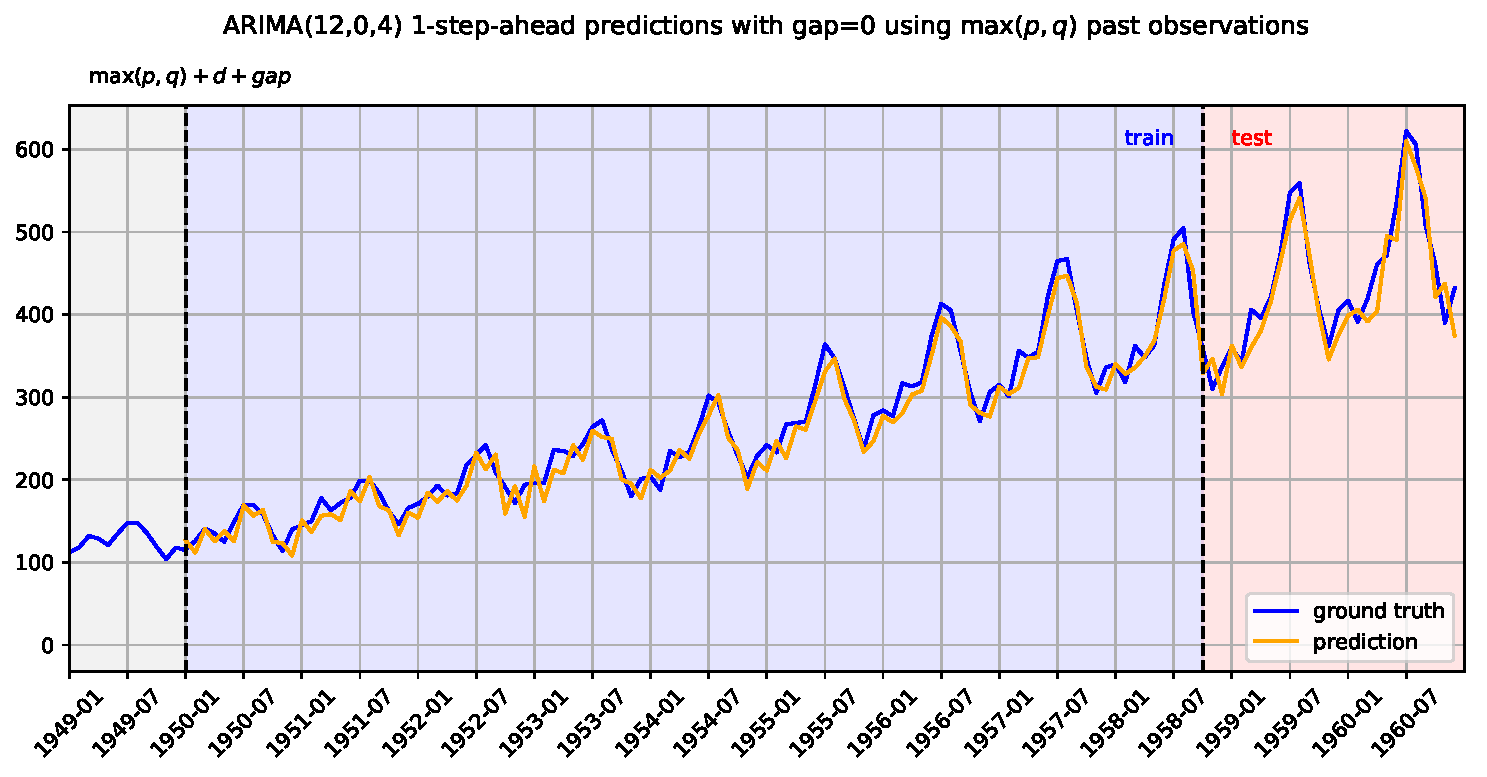
\includegraphics[scale=0.33]{figures/fig1}
    \caption{}
    \label{fig:f1}
  \end{subfigure}

  \begin{subfigure}{\textwidth}
    \centering
    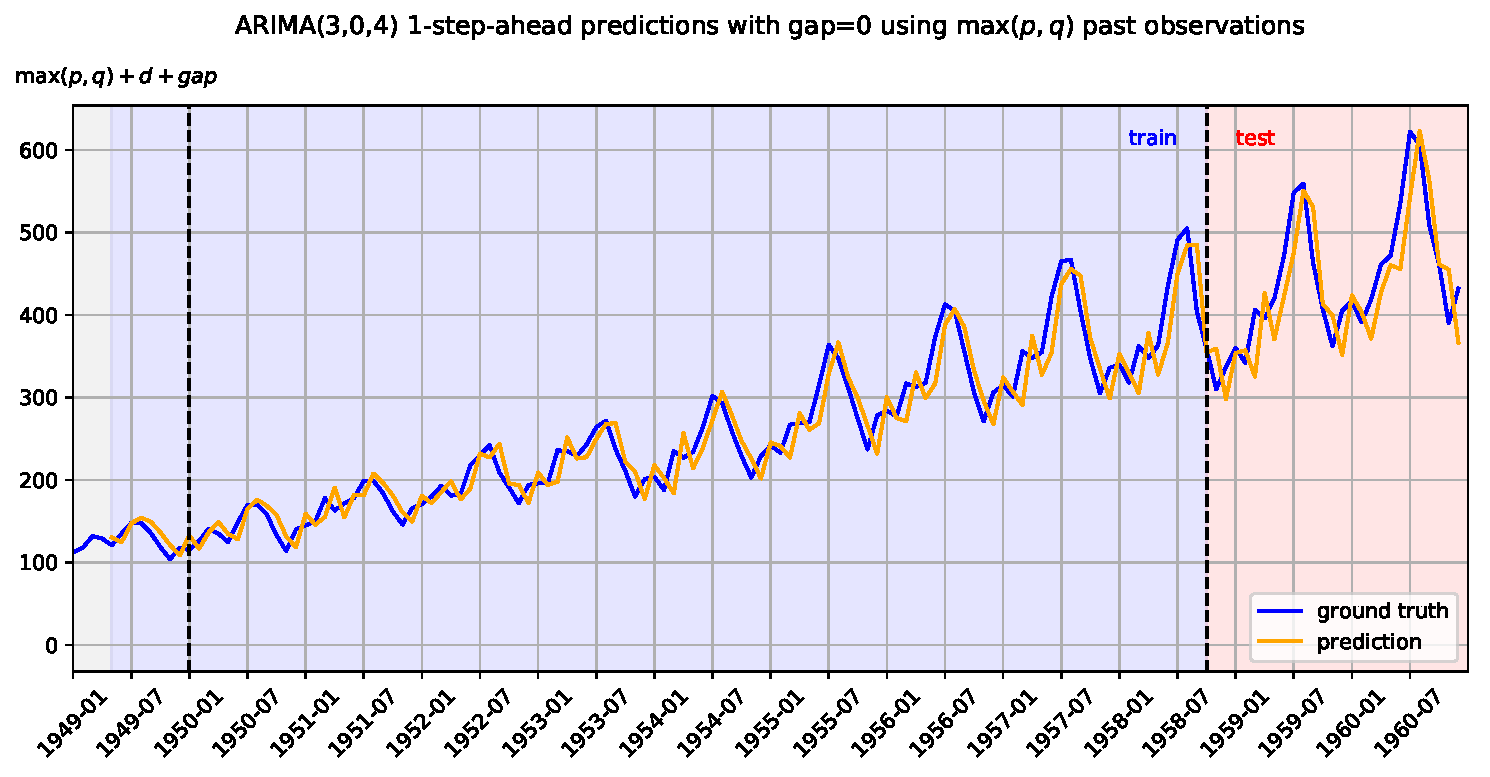
\includegraphics[scale=0.33]{figures/fig2}
    \caption{}
    \label{fig:f2}
  \end{subfigure}

  \begin{subfigure}{\textwidth}
    \centering
    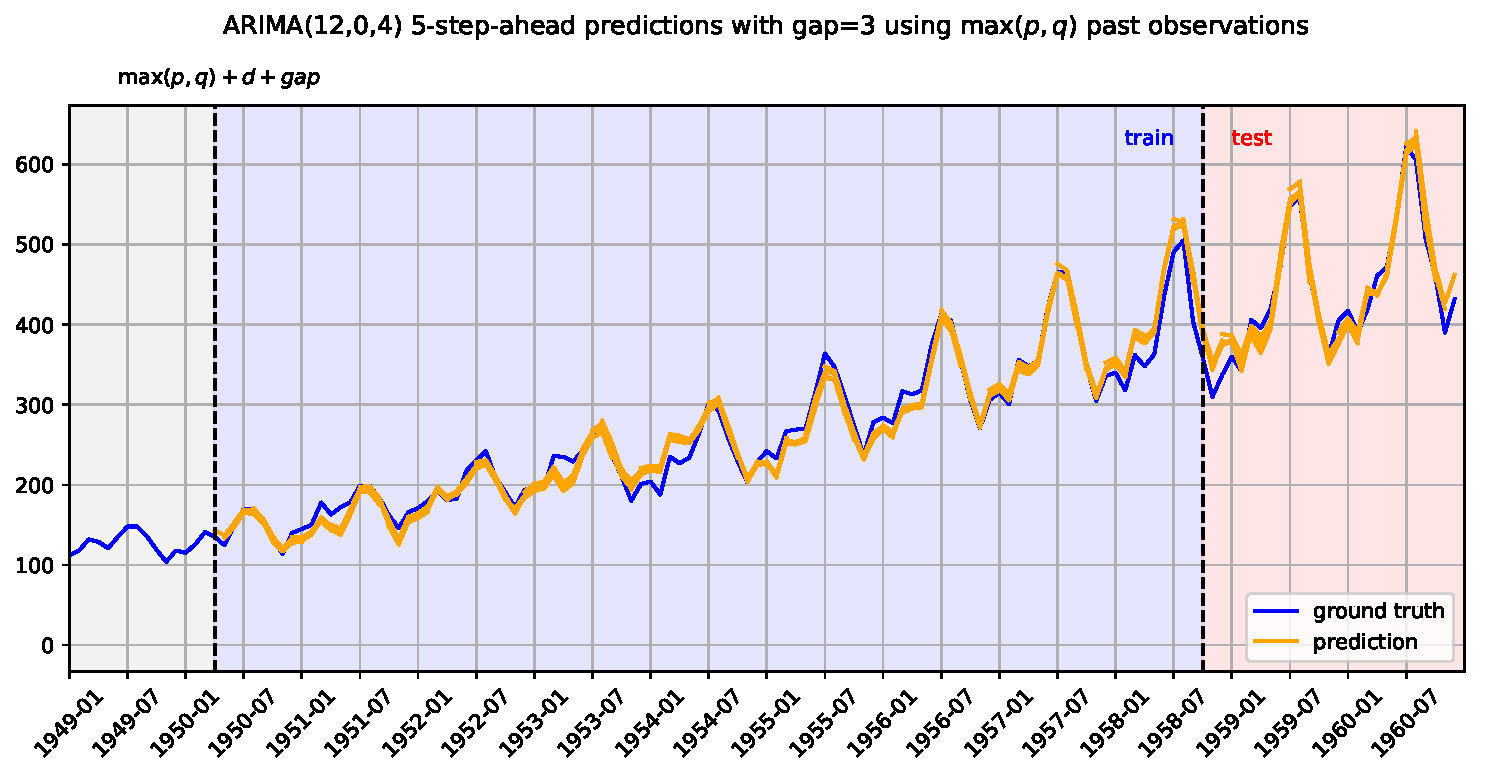
\includegraphics[scale=0.33]{figures/fig3}
    \caption{}
    \label{fig:f3}
  \end{subfigure}

  \caption{results on passengers series using (\ref{fig:f1}) ARIMA(12,0,4) and (\ref{fig:f2}) ARIMA(3,0,4) with g=0 ({\fontfamily{pcr}\selectfont prediction\_gap}), h=1 ({\fontfamily{pcr}\selectfont prediction\_horizon}), trained on 75\% data (until 1958-01). Both train and test set predictions are shown in orange (ground truth is in blue). First actual prediction is at $\max(p,q)+1$. One can note that ARIMA(3,0,4) behaves like the persistence model (i.e., uses the previous value as the prediction for the future). (\ref{fig:f3}) shows ARIMA(12,0,2) for g=3, h=5, i.e. predicting $y_{t+4}, \dots, y_{t+8}$ at once, starting from $\max(p,q)+g+1$.}
  \label{fig:fig1}
\end{figure}



\section{ARIMA}
\subsection{Differencing}
\label{diff}
Differencing removes the changes in the level of a time series, eliminating trend and seasonality and consequently stabilising the mean of the time series. It is usually applied when the raw series in non-stationary, as a means to "stationarise" it (order 1, then 2), and handled in MLCore by {\fontfamily{pcr}\selectfont DeltaTransform1d}.

The classical definition of ARIMA usually considers $\delta=1$ (with order $d=$1 or 2 and rarely above), but in theory, nothing prevents from using larger values e.g., 5-day 7th order differences. As a matter of fact, our ARIMA supports differentiating series using any $\delta$ and $d$, though legitimately, one should then be careful about the nature of the resulting data to be modeled\footnote{as of now, $\delta$ is hard-coded to 1 and $d$ is a free parameter that should not go over 2 (it is difficult to put a physical meaning behind those larger values).}.

Given $d>0$ and $\delta>0$, we introduce the differentiation operator, $D$ in relation to the lag operator from footnote 2, such that $\mathcal{D}_{\delta}^d=\mathcal{D}_{\delta}^1 \circ \mathcal{D}_{\delta}^1 \circ \dots \circ \mathcal{D}_{\delta}^1 \textmd{ (d times)}= (1-L^{\delta})^d$, where $d$ refers to the number of applications of $\mathcal{D}^1_{\delta}$ and $\delta$ is the chosen lag. \\

For example, one can verify that for $t>d\delta$:
\begin{itemize}
  \item
  $
  \mathcal{D}_{\delta}^1y_t=(1-L^{\delta})y_t=y_t-y_{t-\delta}
  $ 
  \item
  $
  \begin{aligned}[t]
    \mathcal{D}_{\delta}^2y_t &= \mathcal{D}_{\delta}^1(\mathcal{D}_{\delta}^1y_t)\\
                  &= (1-L^{\delta})(y_t-y_{t-\delta})\\
                  % &= y_t-y_{t-\delta}-(y_{t-\delta}-y_{t-2\delta})\\
                  &= y_t -2y_{t-\delta} + y_{t-2\delta}
  \end{aligned}
  $
\end{itemize}

From there, one can notice the pattern\footnote{the coefficients of $\mathcal{D}^d_{.}$ (in absolute value) are given by the $d+1$-th row of Pascal's triangle.} that leads to a general expression of the "delta series", $\mathcal{D}_{\delta}^dy$ as a function of $d$ and sequences of $d+1$ terms from the original series $y$: 

\begin{equation}
  \label{eq4}
  \mathcal{D}_{\delta}^dy_t = \sum_{i=0}^d (-1)^i \binom{d}{i} y_{t-i\delta} \textmd{ for } t>d\delta
\end{equation}

In practice, reversing a delta series only requires (i) the order of differentiation (which gives all the coefficients) and (ii) an interleave sequence, $s=y_1, \dots, y_{d\delta}$ made of $\delta$ subseries $s_k=y_{k+i\delta}$ ($0<k\leq \delta$, $0\leq i<d$), each of which allows to recursively compute the unknown term left in eq.~(\ref{eq4}).

For example: given that $\mathcal{D}_3^2 y_t$ is only defined for $t>6$, the first back-transformed term is $y_7 = \mathcal{D}_3^2y_7 + 2\textcolor{blue}{y_4} - \textcolor{blue}{y_1}$. This "round of initialisation" holds for $\mathcal{D}_3^2y_8$ and $\mathcal{D}_3^2y_9$ here (and in general for the first $\delta$ terms), since they use $s_2=\textcolor{blue}{y_2}, \textcolor{blue}{y_5}$ and $s_3=\textcolor{blue}{y_3}, \textcolor{blue}{y_6}$ respectively ($s_1=\textcolor{blue}{y_1}, \textcolor{blue}{y_4}$). Those 3 series are the $\delta$ subseries of the interleave sequence $s=\textcolor{blue}{y_1}, \dots, \textcolor{blue}{y_6}$ defined above. The next terms are obtained in a sliding window fashion.



\begin{figure}
  \centering
  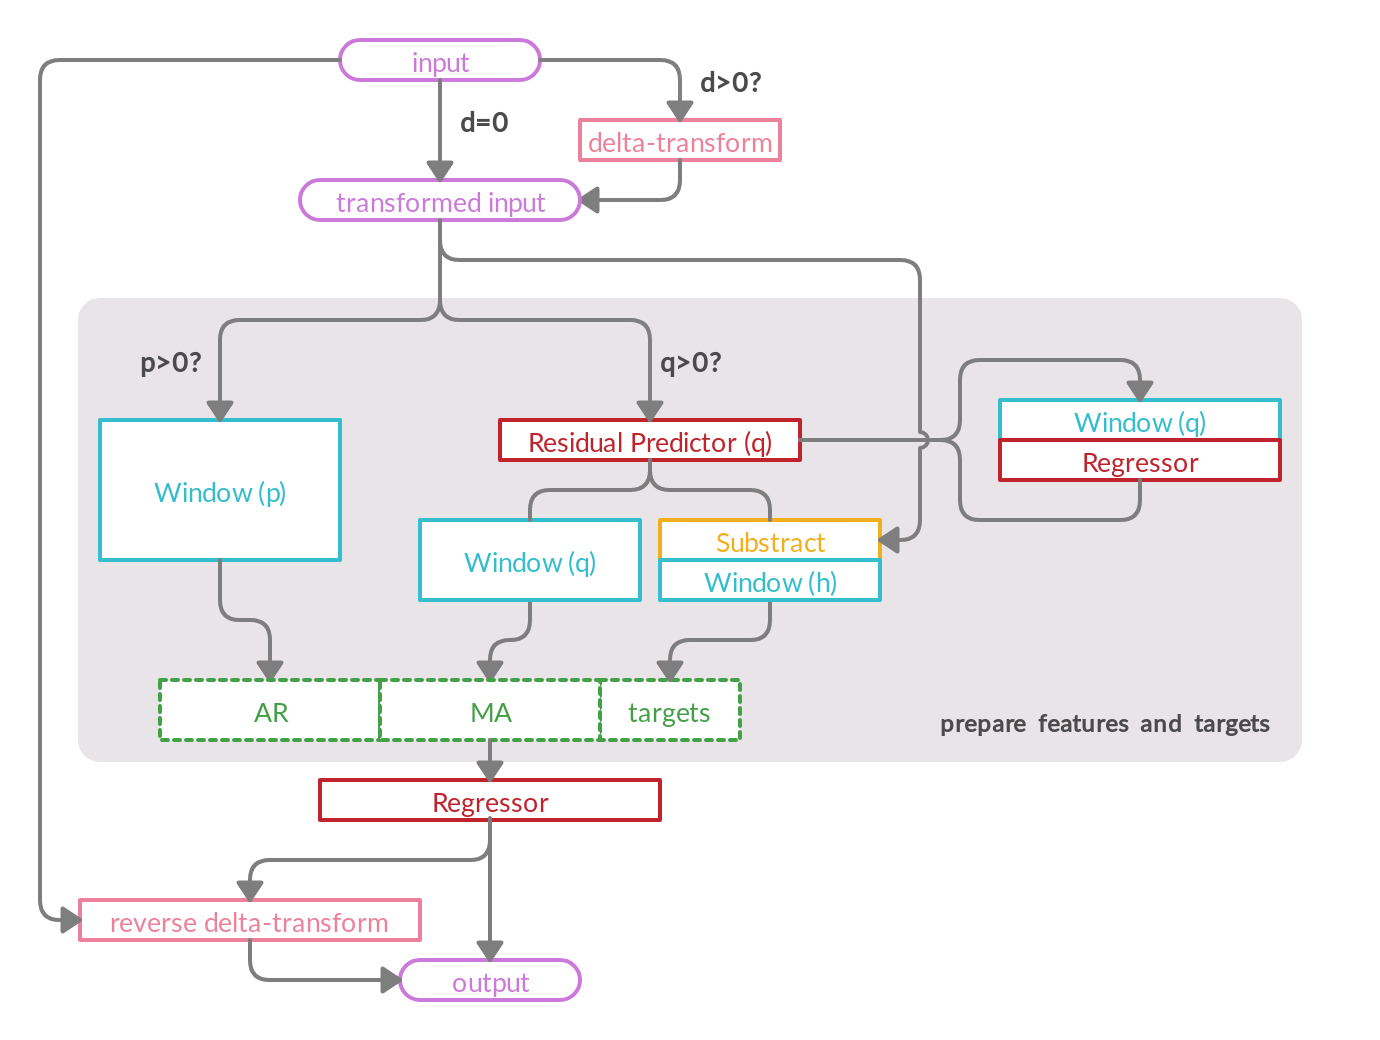
\includegraphics[scale=0.2]{figures/summary}
  \caption{ARIMA flow chart}
  \label{fig:fig4}
\end{figure}



\begin{figure}
  \centering
  \begin{subfigure}{\textwidth}
    \centering
    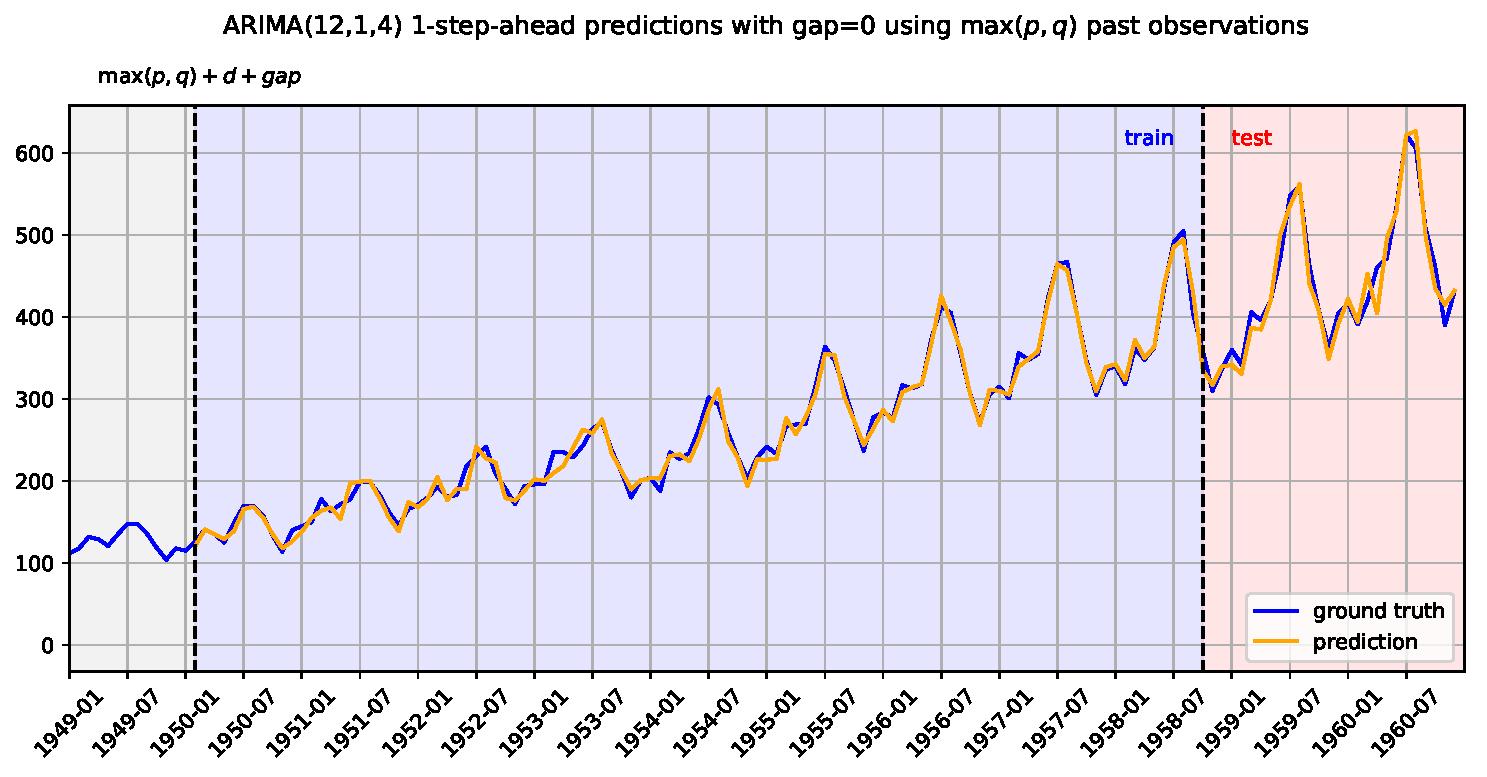
\includegraphics[scale=0.33]{figures/fig4}
    \caption{}
    \label{fig:f4}
  \end{subfigure}

  \begin{subfigure}{\textwidth}
    \centering
    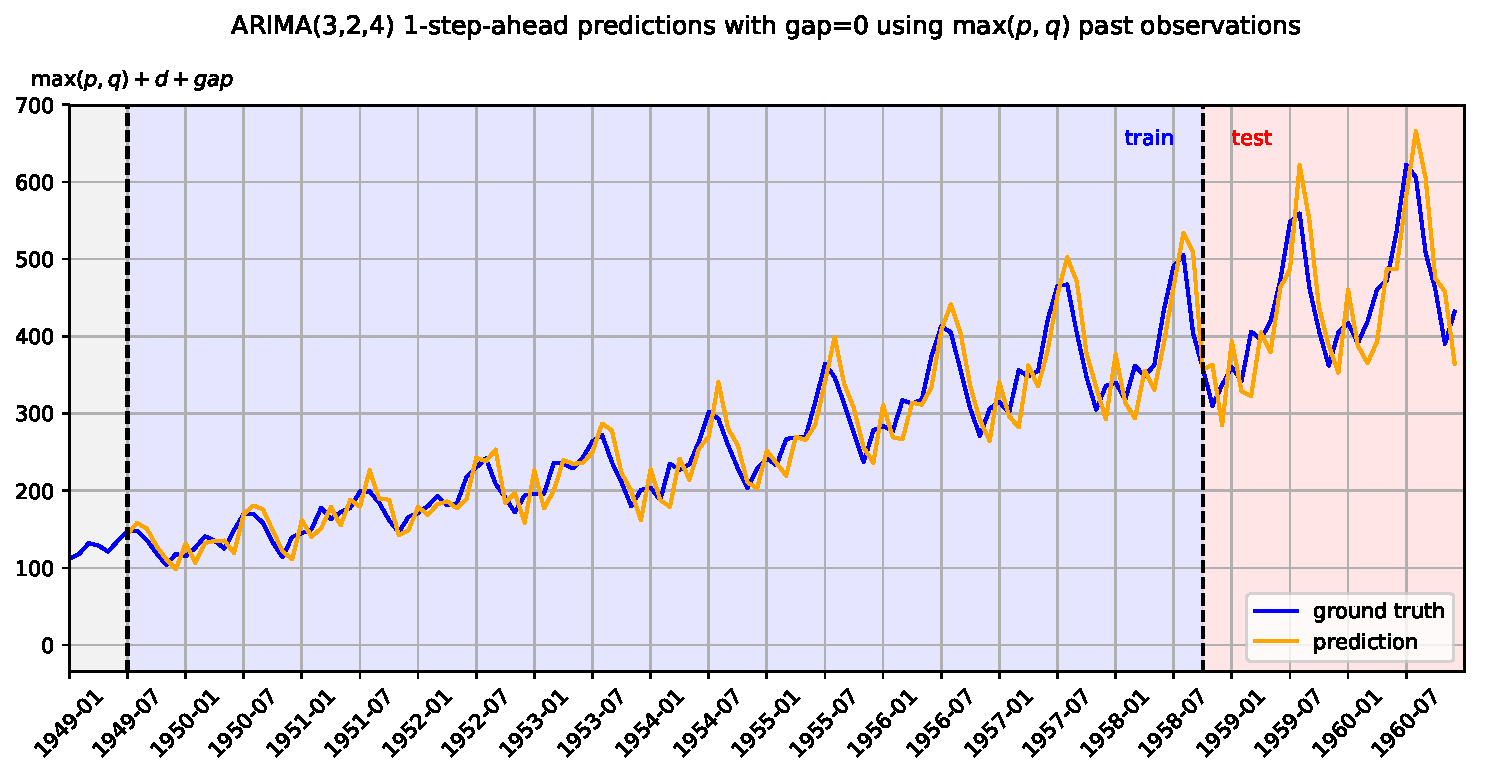
\includegraphics[scale=0.33]{figures/fig5}
    \caption{}
    \label{fig:f5}
  \end{subfigure}

  \begin{subfigure}{\textwidth}
    \centering
    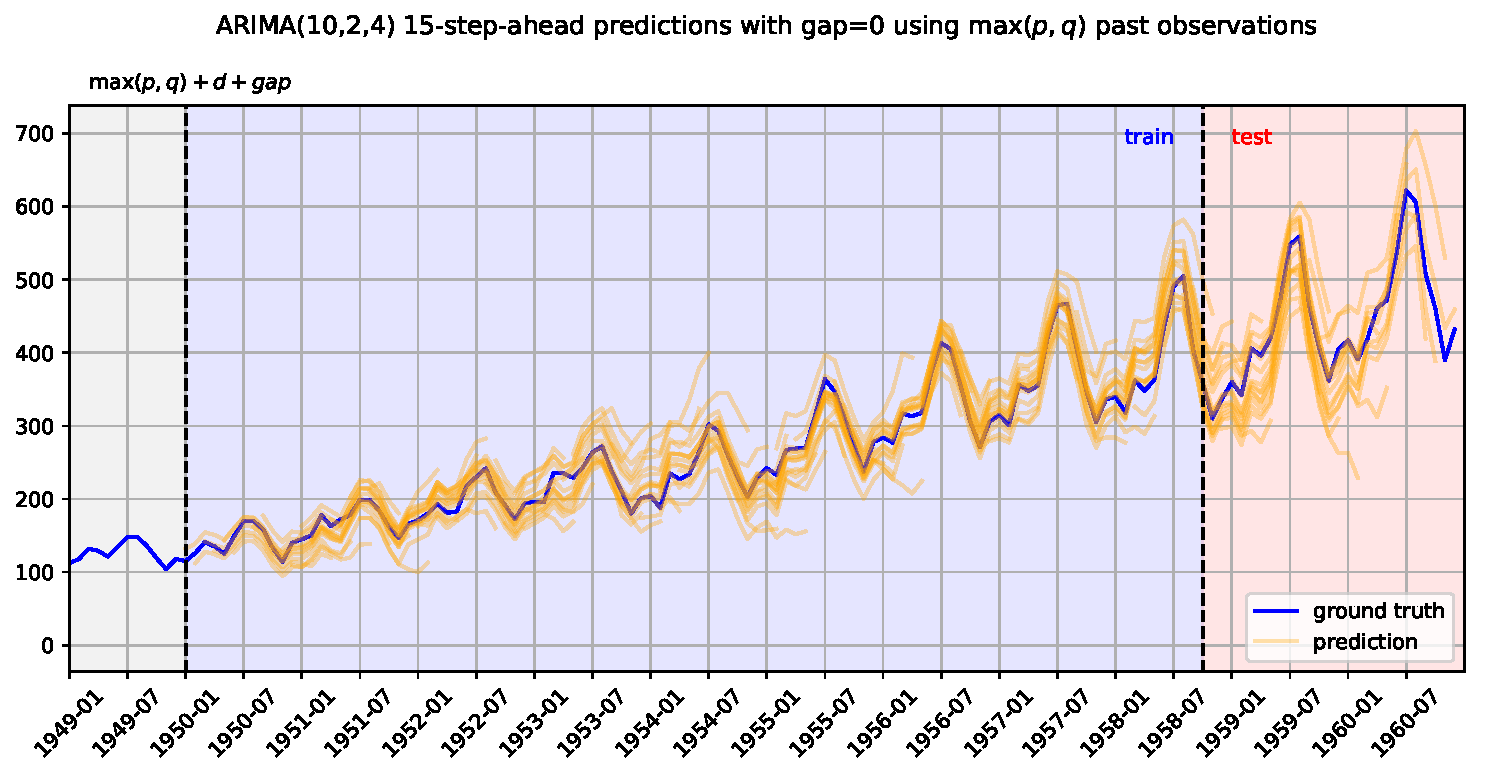
\includegraphics[scale=0.33]{figures/fig6}
    \caption{}
    \label{fig:f6}
  \end{subfigure}

  \caption{results on passengers series using (\ref{fig:f4}) ARIMA(12,1,4) and (\ref{fig:f5}) ARIMA(3,2,4) with g=0 ({\fontfamily{pcr}\selectfont prediction\_gap}), h=1 ({\fontfamily{pcr}\selectfont prediction\_horizon}). (\ref{fig:f6}) shows ARIMA(10,2,4) for g=0, h=15.}
  \label{fig:fig2}
\end{figure}



\subsection{General comments}
As mentioned previously, our ARIMA supports the use of a prediction gap, $g$. Because reconstruction of differentiated series relies on the knowledge of directly preceding terms, ARIMA(p, d>0, q) is incompatible with $g>0$ (or one would have to also predict the target(s)---in the sense of footnote 1---within that gap in order to be able to reverse actual "delta-target(s)" starting at $g+1$; this however goes against the whole point of choosing a non-null value for $g$). 

The following use cases are therefore recommended for any $p,d$ non both null, and any prediction horizon, $h>0$:

\begin{itemize}
\item $d=0$, $g>0$: the model is trained to predict $h$ time points ahead ($y_{t+g+1}, \dots, y_{t+g+h}$)
\item $d>0$, $g=0$: if one is only interested in predicting $y_{t+h}$ using differencing (i.e., $g=h-1$), the model must be trained to predict all $h$ time points ahead ($y_{t+1}, \dots, y_{t+h}$), i.e. forcing $g=0$, from which $y_{t+h}$ may be cherry picked. 
\end{itemize}


\subsection{Summary}
A flow chart is presented in Fig.~\ref{fig:fig4}.


\subsection{Results}
Results are presented in Fig.~\ref{fig:fig2}.

\section{Forecasting}
\subsection{Restrictions}
The following use cases\footnote{a day is used as an arbitrary time unit for the example.} are recommended (distinction between prediction horizon, $h_p$ and forecast horizon, $h_f$ is made here\footnote{note that when $h_f=1$, forecast horizon and prediction horizon are equivalent notions.}):

\begin{itemize}
\item $h_p=1$, $h_f=1$: the model is trained to predict 1 time point ahead; one can then get a 1 day forecast ($h_f$) using the latest window of observations (\textcolor{green}{direct way}).

\item $h_p=7$, $h_f=7$: the model is trained to predict 7 time points at once; one can then get a 7 day forecast using the latest window of observations (\textcolor{green}{direct way}).

\item $h_p=1$, $h_f=7$: the model is trained to predict 1 time point; one can then get a 7 day forecast using previously forecasted values in a sliding fashion (\textcolor{red}{recursive way}). Note that the first sliding window is made of the latest observations; it then slides and gets postpended with forecasts. One should thus be aware that errors will accumulate in this setting.

\item $h_p=7$, $h_f=15$: the model is trained to predict 7 days; one can then get a 15 day-ahead forecast corresponding to forecasting 3 times 1 week, by reusing the forecasted days in a sliding fashion (\textcolor{red}{recursive way}). It is similarly to the previous case except 7 days are predicted at each iteration. Hence diagonal averaging is preformed on the "forecast matrix" to recover a 15 day-ahead forecast vector. Errors will accumulate like in the previous case.
\end{itemize}


\begin{figure}
  \centering
  \begin{subfigure}{0.5\textwidth}
    \centering
    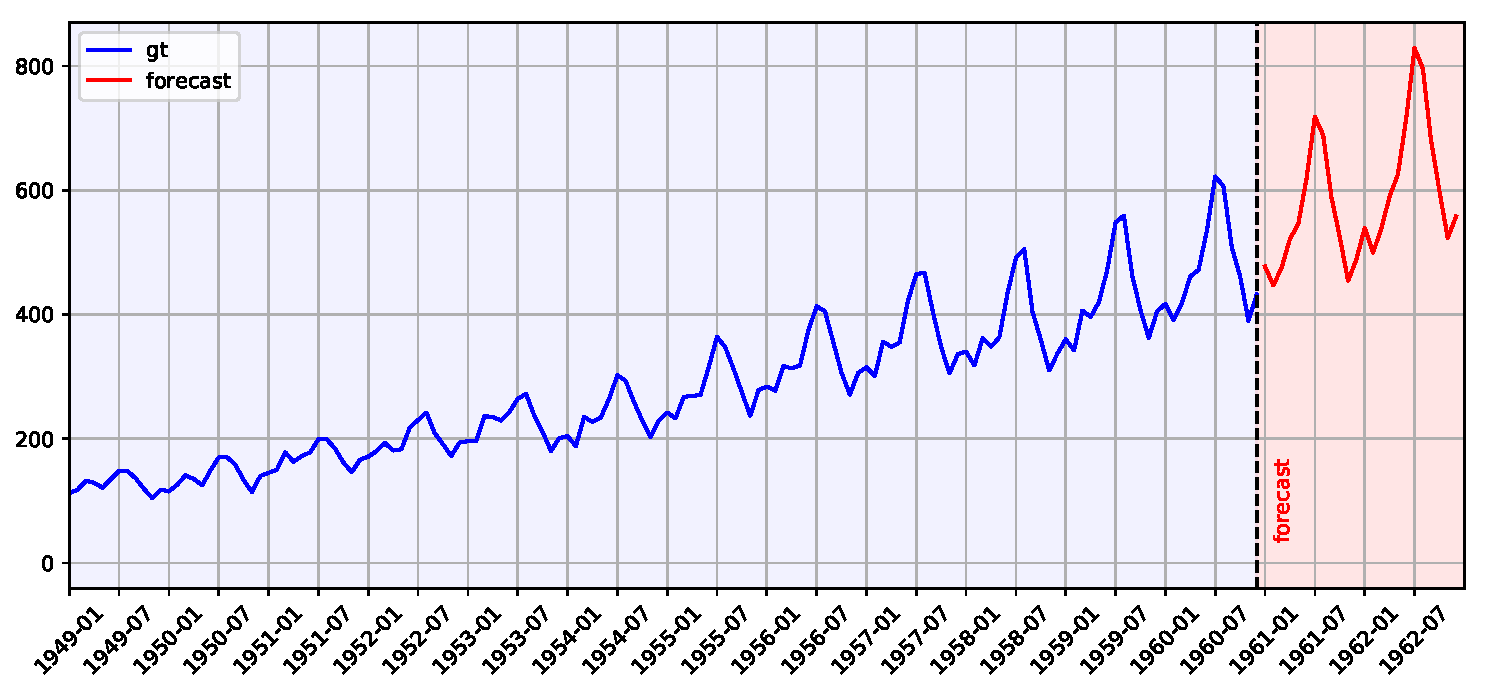
\includegraphics[scale=0.23]{figures/fig7}
    \caption{}
    \label{fig:f7}
  \end{subfigure}%
  \begin{subfigure}{0.5\textwidth}
    \centering
    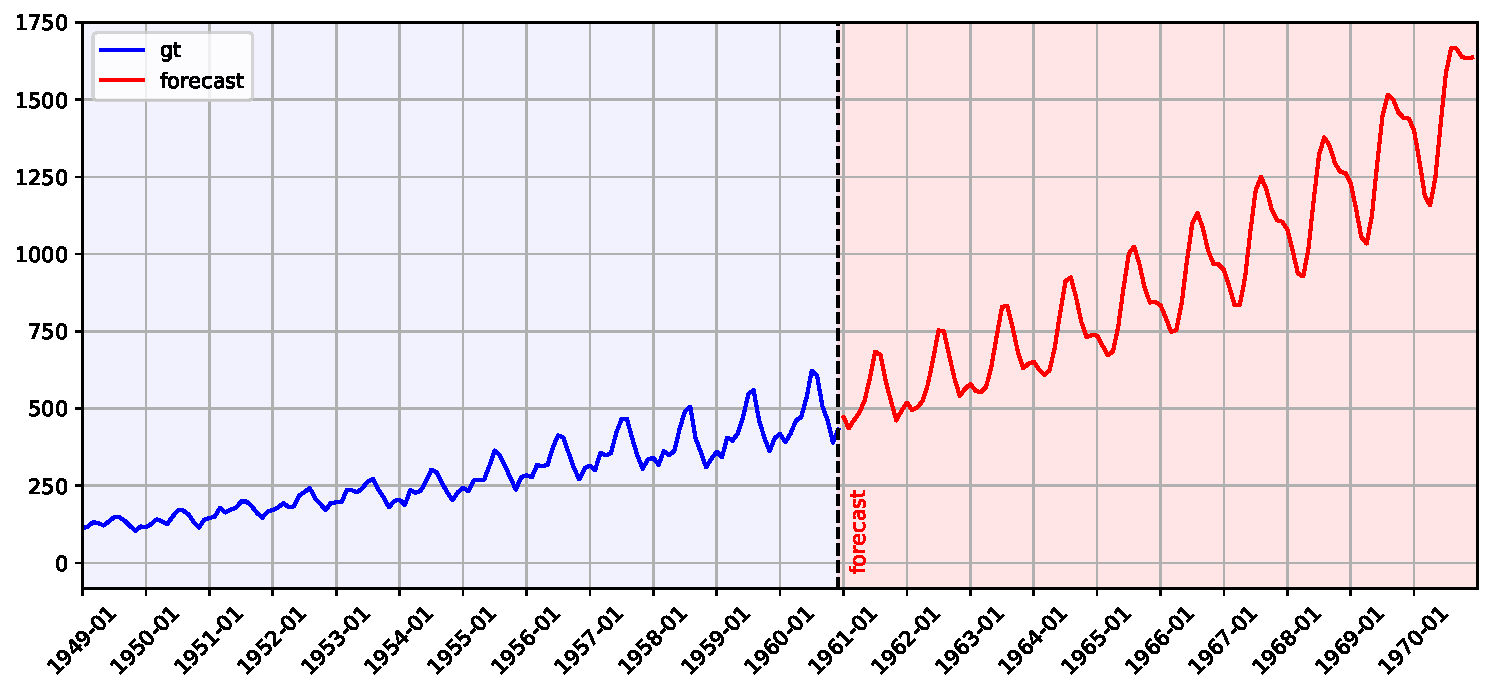
\includegraphics[scale=0.23]{figures/fig8}
    \caption{}
    \label{fig:f8}
  \end{subfigure}


  \begin{subfigure}{0.5\textwidth}
    \centering
    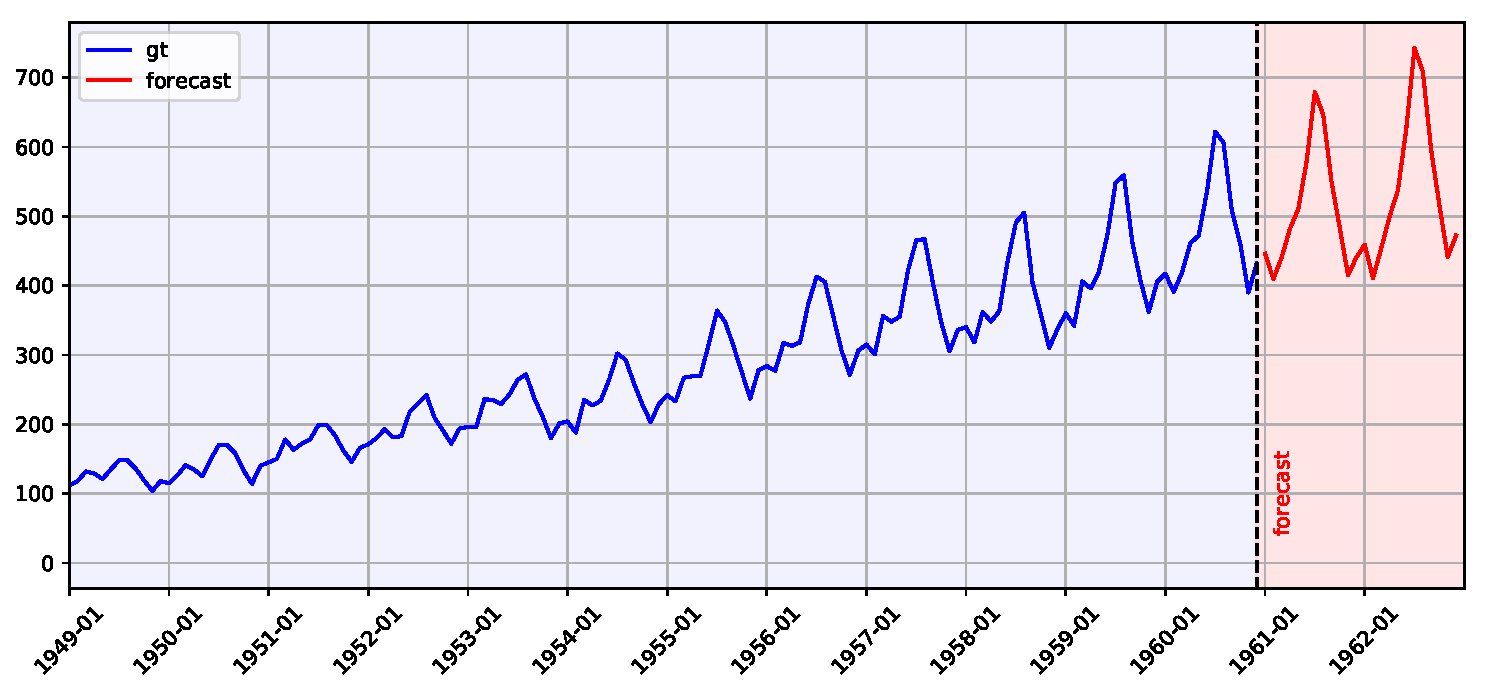
\includegraphics[scale=0.23]{figures/fig9}
    \caption{}
    \label{fig:f9}
  \end{subfigure}%
  \begin{subfigure}{0.5\textwidth}
    \centering
    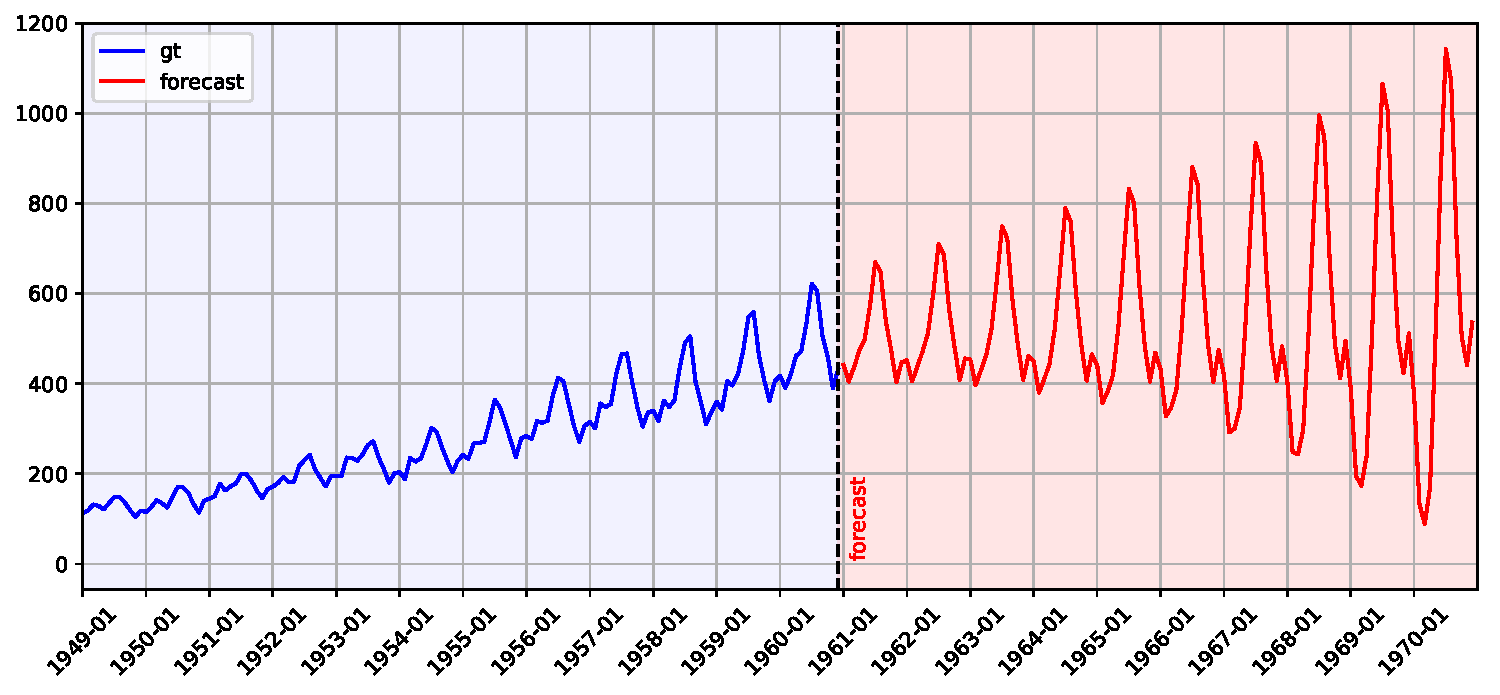
\includegraphics[scale=0.23]{figures/fig10}
    \caption{}
    \label{fig:f10}
  \end{subfigure}

  \begin{subfigure}{0.5\textwidth}
    \centering
    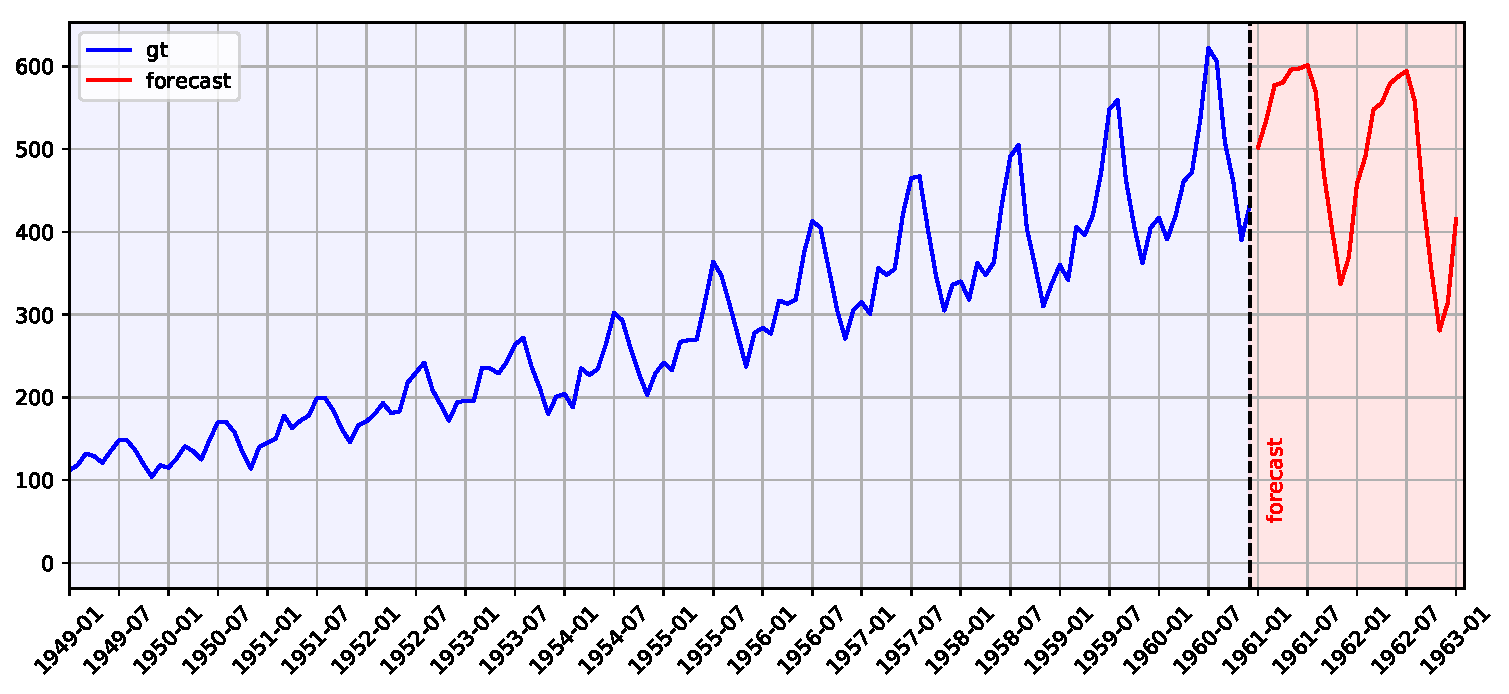
\includegraphics[scale=0.23]{figures/fig12}
    \caption{}
    \label{fig:f12}
  \end{subfigure}%
  \begin{subfigure}{0.5\textwidth}
    \centering
    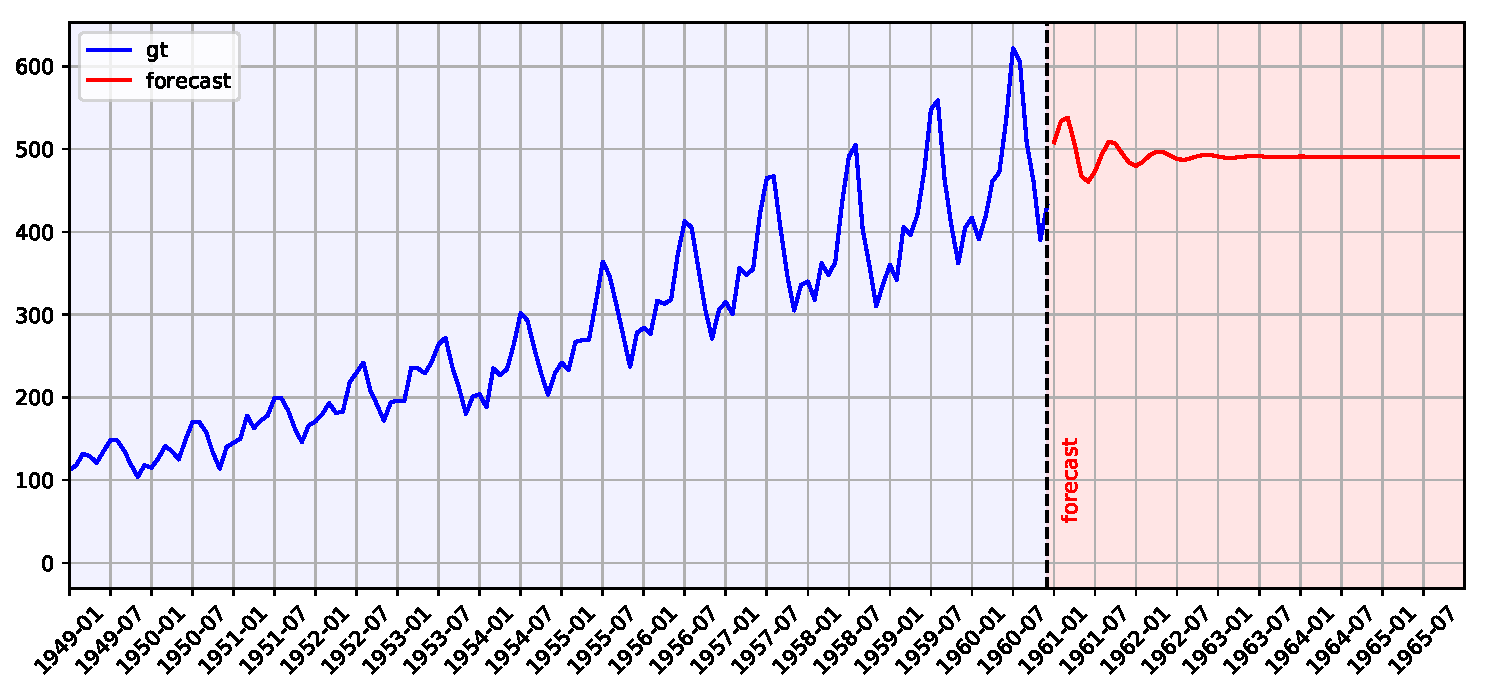
\includegraphics[scale=0.23]{figures/fig11}
    \caption{}
    \label{fig:f11}
  \end{subfigure}


  \caption{results on passengers series using (\ref{fig:f7}) ARIMA(12,0,5) and (\ref{fig:f8}) ARIMA(12,0,5) with $h_p$=24, $h_f=h_p$ (direct way) and $h_p$=1, $h_f$=120 (recursive way) respectively (g=0). (\ref{fig:f9}) and (\ref{fig:f10}) show ARIMA(12,1,5) and ARIMA(12,2,5) with $h_p$=24, $h_f=h_p$ and $h_p$=1, $h_f$=30 respectively. Finally, (\ref{fig:f12}) and (\ref{fig:f11}) show ARIMA(3,1,5) with $h_p$=25, $h_f=h_p$ and $h_p$=1, $h_f$=60 respectively.}
  \label{fig:fig3}
\end{figure}


\subsection{Results}
Results are presented in Fig.~\ref{fig:fig3}.



\end{document}